\chapter{Orbiting Hot Spots: the GRAVITY Flares}
\label{ch:xflares}

Several times a day the near-infrared emission of \sgra{} flares, rising
within minutes to many times its quiescent level \citep{Genzel2010}. In 2018
the GRAVITY interferometer resolved the motion of three bright flares
\citep{Gravity2018flares}. Their emission centroids traced clockwise loops on
the sky, with the polarisation angle rotating in step. On July~22 the
centroid moved by about 120\,$\muas$ in about 30 minutes, roughly 30 per cent
of the speed of light. GRAVITY's relativistic modelling located the emitter on
a near face-on circular orbit just outside the innermost stable orbit, with
best fits near $R \approx 7\pm0.5\,R_g$, $i \approx 160\degr\pm10\degr$ and a
period $P = 40\pm8$ minutes. The other two flares traced loops of total
amplitude $\sim$110--140\,$\muas$. A dedicated follow-up
\citep{Gravity2020flares} found all three flares consistent with a compact
hot spot at $R \approx 9\,R_g$ and $i \approx 140\degr$, and noted a tension:
the observed motion on the sky is systematically \emph{larger} than geodesic
hot-spot models predict for the observed period.

This chapter builds that model on our \sgra{} spacetime, traces it with full
slow-light ray tracing, and compares its observables with the published
ones. Every orbit and inclination below is taken from those papers; nothing
is tuned.

\section{The model}

The emitter is the one GRAVITY used \citep[][following
\citealt{BroderickLoeb2006, Hamaus2009}]{Gravity2020flares}: a Gaussian blob
of emissivity $\varepsilon \propto \exp(-d^2/2s^2)$, size $s = \XFlSigma\,M$
(their fiducial value), whose centre follows the prograde circular equatorial
geodesic of BL radius $R$, $\Omega = 1/(R^{3/2} + a)$. The blob moves rigidly
with the centre's 4-velocity $u = u^t(\partial_t + \Omega\,\partial_\phi)$, and
$d$ is the comoving distance $d^2 = (g_{\mu\nu} + u_\mu u_\nu)\,\Delta x^\mu
\Delta x^\nu$ at fixed coordinate time. The emission is optically thin, with
$j_\nu \propto \nu^{-\alpha}$. Along a backward ray normalised so the camera
measures unit frequency, conservation of $I_\nu/\nu^3$ gives
\begin{equation}
I_{\rm obs} = \int g^{2+\alpha}\,\varepsilon\,d\lambda, \qquad
g = \frac{1}{u^t\,(p_t + \Omega L_z)},
\label{eq:spotintensity}
\end{equation}
where $g$ is one number per ray for a rigidly rotating emitter. With
$\alpha = 0$ this is exactly the GRAVITY 2020 prescription, $F = \int D^2
\varepsilon\,ds$. The value $\alpha = 0.6$, one of the spectral indices
GRAVITY used to illustrate beaming \citep[their Appendix
C]{Gravity2018flares}, measures the sensitivity to that choice.

\emph{Slow light.} Each ray carries its Kerr--Schild time
(Chapter~\ref{ch:xks}). Light reaching the camera at observing time
$t_{\rm obs}$ left a point on the ray at $t_{\rm obs} + \Delta t$, when the spot
was where it was then. The simulator does not freeze the source while the
light travels.

\emph{Ray table.} The spacetime is stationary, so each pixel's ray is traced
once (fp64, adaptive Dormand--Prince) from a camera at $1000\,M$ over a field
of $\pm\XFlHalfWidth\,M$ with $\XFlPixels^2$ pixels. The tracer stores every
sample within $6s$ of the orbit, at a spacing of at most $s/5$, together with
its Kerr--Schild time and its image order: 0 for the direct image, 1 for the
first image lensed around the hole. Any observing time and emission model is
then a sum over stored samples. Along all rays $|H|/E^2 \le \XFlMaxdH$ and
the relative drift of $L_z$ is $\le \XFlMaxdL$.

\emph{Tests} (\texttt{test\_hotspot.cpp}) cover four properties:
\begin{itemize}
\item the orbit closes after exactly $2\pi(R^{3/2} + a)$;
\item the comoving distance co-rotates with the spot;
\item the Kerr--Schild light-travel time matches Carter's $t$-equation
(Chapter~\ref{ch:xks});
\item cameras at $i$ and $180\degr - i$ record identical light curves and
mirror-image centroid tracks, as the equatorial symmetry of Kerr requires.
\end{itemize}

\emph{Numerical noise.} The lensed images are thin arcs that no affordable
grid resolves. As they move across pixels they add a pixel-scale jitter that
shrinks as $1/n$. All observables below use the first twelve harmonics of the
one-orbit series, which removes $\XFlGraNoiseFlux$\,\% (rms) from the light
curve and $\XFlGraNoiseCentroid\,\muas$ from the centroid track. At half the
resolution ($\XFlResHalf^2$ pixels) the loop size changes by $\XFlResLoop$\,\%,
the flux contrast by $\XFlResContrast$\,\% and the echo delay by
$\XFlResEcho$\,\%. These are the numerical uncertainties of the values below.

\section{Comparison with GRAVITY}

Table~\ref{tab:xflares} and Figure~\ref{fig:xflarecurves} give the results
for three orbits:
\begin{itemize}
\item GRAVITY's 2018 best fit;
\item their 2020 global fit;
\item the radius whose prograde period, for our spin and the GRAVITY 2022
mass, equals the 2018 best-fit period of 40 minutes ($R = \XRPforty\,M$).
\end{itemize}

\begin{table}
\centering
\caption{Simulated observables of an orbiting hot spot around \sgra{}
($\astar = 0.94$; $s = \XFlSigma\,M$), from \texttt{flare\_tool}. Loop: the
largest separation of two centroid positions; in brackets the geometric
orbit diameter. Chord: the largest centroid displacement within 30
minutes and the corresponding speed. Contrast: maximum over minimum flux
for $\alpha = 0$ ($\alpha = 0.6$). Lensed: mean flux fraction in images of
order $n \ge 1$. Echo: delay of the $n=1$ image of a flash behind the direct
one, over eight orbital phases.}
\label{tab:xflares}
\small
\begin{tabular}{lccc}
\toprule
& GRAVITY 2018 & GRAVITY 2020 & $P = 40$\,min \\
\midrule
$R$ [$M$], $i$ [deg] & $\XFlGraR$, $\XFlGraIncl$ & $\XFlGrbR$, $\XFlGrbIncl$ & $\XFlPfoR$, $\XFlPfoIncl$ \\
period [min] & $\XFlGraPeriod$ & $\XFlGrbPeriod$ & $\XFlPfoPeriod$ \\
loop [$\muas$] & $\XFlGraLoop$ ($\XFlGraOrbit$) & $\XFlGrbLoop$ ($\XFlGrbOrbit$) & $\XFlPfoLoop$ ($\XFlPfoOrbit$) \\
30-min chord [$\muas$] ($c$) & $\XFlGraChord$ ($\XFlGraChordSpeed$) & $\XFlGrbChord$ ($\XFlGrbChordSpeed$) & $\XFlPfoChord$ ($\XFlPfoChordSpeed$) \\
contrast & $\XFlGraContrast$ ($\XFlGraContrastSix$) & $\XFlGrbContrast$ ($\XFlGrbContrastSix$) & $\XFlPfoContrast$ ($\XFlPfoContrastSix$) \\
lensed flux [\%] & $\XFlGraLensed$ & $\XFlGrbLensed$ & $\XFlPfoLensed$ \\
echo delay [min] & $\XFlGraEchoMinMin$--$\XFlGraEchoMaxMin$ & $\XFlGrbEchoMinMin$--$\XFlGrbEchoMaxMin$ & $\XFlPfoEchoMinMin$--$\XFlPfoEchoMaxMin$ \\
\bottomrule
\end{tabular}
\end{table}

\begin{figure}
\centering
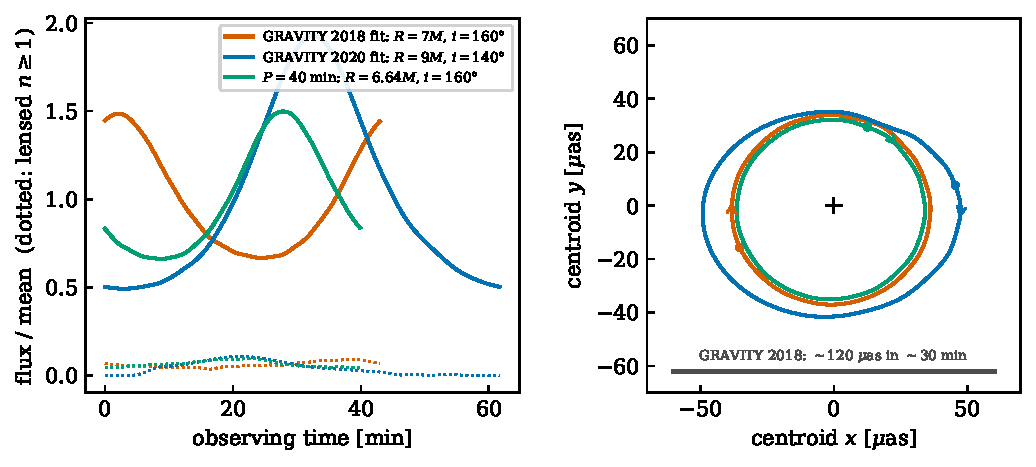
\includegraphics[width=\textwidth]{figures/fig_x_flare_curves.pdf}
\caption{Hot spots on the GRAVITY orbits around \sgra{}. Left: light curves
over one orbit, normalised to the mean (dotted: the part carried by lensed
images). Right: the flux-weighted centroid tracks on the sky (dot: start;
arrows: sense of motion; cross: the black hole). The grey bar shows the
centroid motion GRAVITY measured in the July 2018 flare, about 120\,$\muas$ in
about 30 minutes \citep{Gravity2018flares}.}
\label{fig:xflarecurves}
\end{figure}

\paragraph{Period and sense.} On GRAVITY's 2018 orbit the spot circles
\sgra{} in $\XFlGraPeriod$ minutes, inside the measured $40\pm8$. Seen from
$i > 90\degr$ its motion is \XFlGraSense{} on the sky, as observed. The 2020
orbit, at $9\,M$, takes $\XFlGrbPeriod$ minutes: within the 33--65-minute
range GRAVITY quoted as consistent with all three flares, but longer than the
July~22 best fit. The two radii bracket the problem.

\paragraph{Loop size and speed.} Lensing enlarges the apparent orbit a little
\citep[as GRAVITY's models also show;][]{Gravity2018flares}: the 2018 orbit's
centroid loop measures $\XFlGraLoop\,\muas$ against a geometric diameter of
$\XFlGraOrbit\,\muas$. Within any 30 minutes, however, the centroid moves at
most $\XFlGraChord\,\muas$ ($\XFlGraChordSpeed\,c$), about half the
$\sim$120\,$\muas$ ($\sim$0.3\,$c$) GRAVITY measured in the same interval.
Moving the spot out to $9\,M$ at $i = 140\degr$ brings the 30-minute chord to
$\XFlGrbChord\,\muas$, but at a period of $\XFlGrbPeriod$ minutes. No circular
geodesic reconciles both. This reproduces, with an independent code and our
own spacetime, the tension of \citet{Gravity2020flares}: the observed motion
is faster and larger than a hot spot on a geodesic can be for the observed
period. They discuss two partial explanations, neither modelled here:
astrometric scatter biases a measured radius upward by
$\sqrt{1 + \sigma^2/R^2}$, and the spot may move toward the observer.

\paragraph{Flux contrast.} On the 2018 orbit the light curve varies by a
factor $\XFlGraContrast$ for $\alpha = 0$ ($\XFlGraContrastSix$ for $\alpha =
0.6$). This is the combined effect of Doppler beaming, lensing and the
changing path through the blob. GRAVITY's combined orbit constraints required
a Doppler contrast below about 2.5 \citep[their Fig.~B.3]{Gravity2018flares}:
the 2018 orbit meets that with $\alpha = 0$ and only marginally with
$\alpha = 0.6$. The 2020 geometry, more inclined, varies by
$\XFlGrbContrast$. Its intrinsic heating and cooling would have to mask a
beaming signal of that size. The loop centres lie $\XFlGraOffset\,\muas$ (2018)
and $\XFlGrbOffset\,\muas$ (2020) from the black hole, well inside the
$\pm$50\,$\muas$ within which GRAVITY found them consistent with the mass
centroid.

\section{Photon-ring echoes}

Light from the spot also reaches the camera along a second path, around the
hole, as the thin lensed image in Fig.~\ref{fig:xflareimages}. That image
carries $\XFlGraLensed$ per cent of the flux on average on the 2018 orbit. Because the
second path is longer, a sudden change in the source appears twice. Flashing
the spot briefly ($\tau = 1\,M$) at eight points of its orbit and following
the direct and the first lensed image separately (Fig.~\ref{fig:xecho})
gives echo delays of $\XFlGraEchoMin$--$\XFlGraEchoMax\,M$, that is
$\XFlGraEchoMinMin$--$\XFlGraEchoMaxMin$ minutes (mean $\XFlGraEchoMeanMin$).
The echo peaks at $\XFlGraEchoPeakMin$--$\XFlGraEchoPeakMax$ per cent of the
direct flash. The delay depends on the phase because the extra path depends
on where the spot is relative to the line of sight; at the more inclined 2020
geometry it spans $\XFlGrbEchoMinMin$--$\XFlGrbEchoMaxMin$ minutes. These are
the time-domain counterpart of the thesis' photon-ring analysis: a delay set by
the mass and geometry alone, measurable in principle without resolving the
ring.

\begin{figure}
\centering
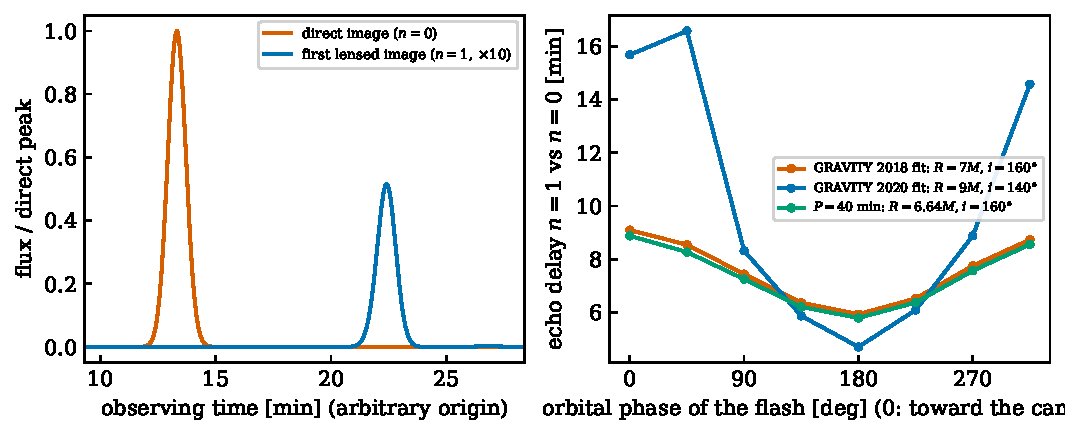
\includegraphics[width=\textwidth]{figures/fig_x_echo.pdf}
\caption{Photon-ring echoes on the GRAVITY 2018 orbit. Left: a brief flash
($\tau = 1\,M$) seen in the direct image and, delayed, in the first lensed image
(scaled up tenfold). Right: the echo delay versus the orbital phase of the
flash for the three orbits of Table~\ref{tab:xflares}.}
\label{fig:xecho}
\end{figure}

\section{The live view}

The live renderer traces the same emitter: the orbit constants and the
comoving metric are computed by the same CPU class and handed to the shader,
and each ray integrates its own Kerr--Schild time. Against the fp64 images at
four orbital phases (\texttt{compare\_flare.py}) the GPU total flux agrees to
$\XFlGpuFluxDev$\,\%, the centroid to $\XFlGpuCentroidPx$\,pixel, and the
image correlation is at least $\XFlGpuCorr$. Figure~\ref{fig:xflareimages}
shows the fp64 images. In the interactive renderer and the movie of one orbit
(\texttt{scripts/make\_flare\_movie.py}) the spot is drawn in false colour,
because 2.2\,$\mu$m synchrotron light has no visible hue.

\begin{figure}
\centering
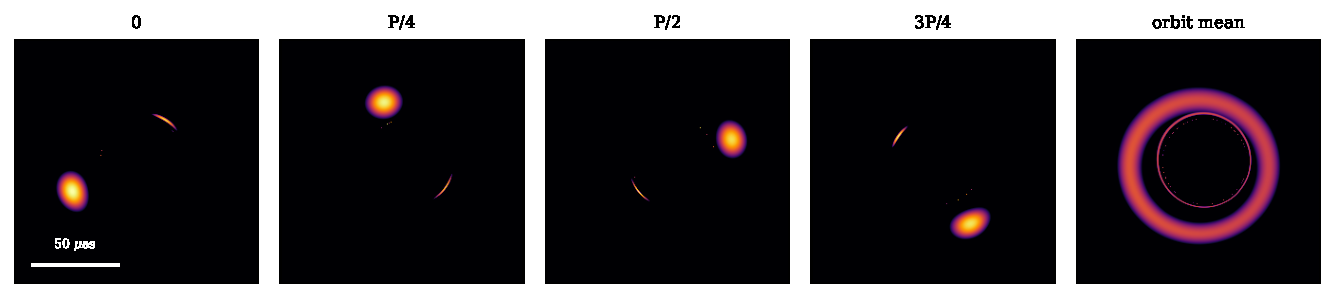
\includegraphics[width=\textwidth]{figures/fig_x_flare_images.pdf}\\[4pt]
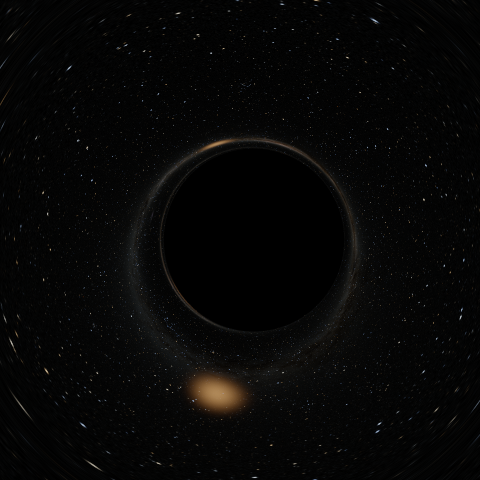
\includegraphics[width=0.24\textwidth]{figures/x_flare_0.png}\hfill
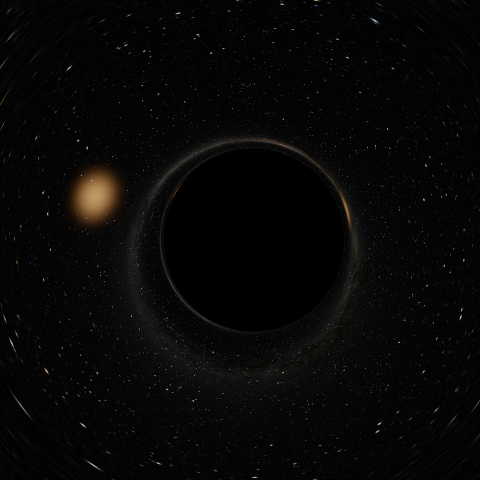
\includegraphics[width=0.24\textwidth]{figures/x_flare_1.png}\hfill
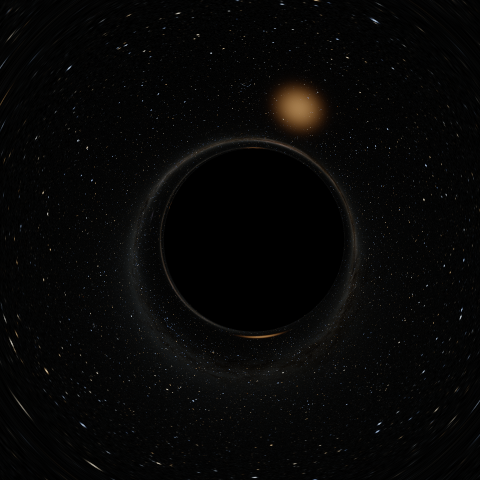
\includegraphics[width=0.24\textwidth]{figures/x_flare_2.png}\hfill
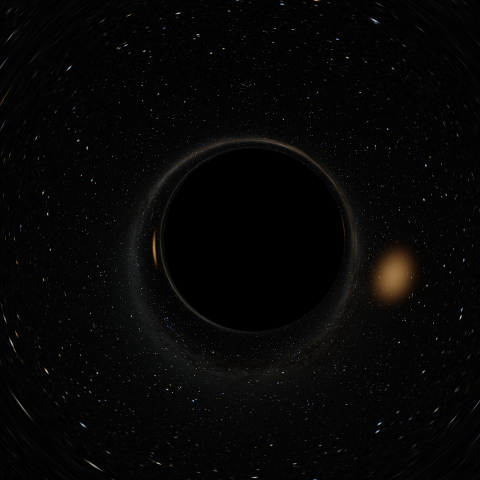
\includegraphics[width=0.24\textwidth]{figures/x_flare_3.png}
\caption{The GRAVITY 2018 hot spot around \sgra{} ($R = 7\,M$, $i = 160\degr$).
Top: fp64 images (logarithmic stretch, four decades) at quarter orbits and
averaged over one orbit; the thin arcs near the shadow edge are the lensed
images. Bottom: the live renderer at the same phases from $45\,M$, with the
lensed Milky Way behind and the spot in false colour.}
\label{fig:xflareimages}
\end{figure}
